\usetikzlibrary{calc}
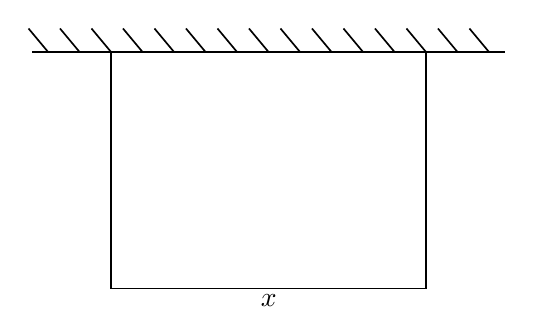
\begin{tikzpicture}[x=1cm,y=1cm,line width=.6pt,font=\normalsize]
% wall
\draw ( -1,3) -- (5,3);
% wall hatch ticks (15), short diagonals above wall
\foreach \x in {-0.8,-0.4,0,0.4,0.8,1.2,1.6,2.0,2.4,2.8,3.2,3.6,4.0,4.4,4.8} {
  \draw (\x,3) -- (\x-0.25,3.3);
}
% three fence sides
\draw (0,3) -- (0,0) -- (4,0) -- (4,3);
% label x below bottom edge centre
\node[inner sep=0pt,anchor=north,yshift=-2pt] at (2,0) {$x$};
\end{tikzpicture}
